\documentclass[12pt]{scrartcl} %Dokumentklasse, bestimmt Teile des Layouts
\usepackage[utf8]{inputenc} %Ermöglicht Unicode, absolut notwendig
\usepackage[ngerman]{babel} %Ermöglicht deutsche Sonderzeichen, z. B. Umlaute
\usepackage[T1]{fontenc} %Ermöglicht Unicode, absolut notwendig
\usepackage{amsmath} %Wichtige Mathe-Möglichkeiten
\usepackage{amssymb} %Wichtige Mathe-Möglichkeiten
\usepackage{epstopdf} %Um .eps-Bilder in Latex verwenden zu können
\usepackage[onehalfspacing]{setspace} %Bestimmt den Zeilenabstand, hier 1,5
\usepackage{graphicx} %Bessere Bilder
\usepackage{array} %Bessere Formatierung / Umgebung für mehrzeilige Formeln
\usepackage{upgreek} %Für nicht kursive griechische Buchstaben, z. B. \upmu statt \mu
\usepackage{float} %Großes H zum fixieren von Abbildungen/Tabellen
%\usepackage{csquotes}% Anführungszeichen etc.
\usepackage{mhchem}% für Chemische Formeln und Reaktionsgleichungen
\usepackage{tikz} %Vektorgrafziken im LaTeX-eigenen Format, z. B. zum Export aus QtiPlot
\usepackage{graphicx}
\usepackage[font=small]{caption} %Bestimmt die Schriftgröße von Tabellenüberschriften und Bildunterschriften, optional
\usepackage[backend=biber, style=chem-angew]{biblatex} %Literaturverzeichnis
\usepackage{tabularx, booktabs, multirow} %Für bessere Tabellen und einfachen Excel to Latex import
\usepackage[
  left=3cm,
  right=2cm
]{geometry}
\usepackage{pgfplots}
\newcommand{\celsius}{^{\circ}\mathrm{C}} %Ermöglicht es, \celsius für die Einheit °C zu verwenden
\geometry{bottom=100pt} \geometry{top=100pt} %Definiert den oberen und unteren Rand, optional
\parindent0pt %Kein Einzug am Anfang von Absätzen
\sloppy %Besserer Blocksatz
\renewcaptionname{ngerman}{\figurename}{Abb.} %Umbenennung Abbildungen, optional
\renewcaptionname{ngerman}{\tablename}{Tab.} %Umbenennung Tabellen, optional
\begin{document}
\begin{titlepage}
\begin{center}
\vspace*{2cm}
\begin{LARGE}
\vspace*{1cm}
\textbf{\textsf{Quantitative Analyse - Aufgabe 5\\}}
\end{LARGE}
\vspace*{1cm}
\textbf{\textsf{Praktikum zur analystischen Chemie}}\\
\vspace*{1.5cm}
\begin{table}[H]
\sffamily
\hspace*{3cm}\begin{tabular}{>{\bfseries}l>{\bfseries}l}
Verfasser: Maxim Gilsendegen\\
Matrikelnummer: 3650677\\
E-Mail-Adresse: 182513@stud.uni-stuttgart.de\\
Assistent: Robert Stelzer\\
Abgabedatum: 19.07.2023\\
\end{tabular}
\end{table}
\end{center}
\end{titlepage}
\renewcommand{\thepage}{\Roman{page}}\setcounter{page}{1}
\tableofcontents %Generiert ein Inhaltsverzeichnis, optional
\newpage
\renewcommand{\thepage}{\arabic{page}}\setcounter{page}{1}

\section{Aufgabe}
Bestimmung der Stoffmenge von Oxalsäure durch Titrieren mit einem $p$H-Meter und analyse der entstehenden Titrationskurve.\\

\section{Durchführung}
Die Titration wurde mit drei Aliquoten durchgeführt. Jeder 25 ml Aliquot wurde in ein 250 ml Becherglas gegeben und ein $p$H-Meter in die Lösung getaucht, diese wurde dann aufgefüllt, bis die Elektrode komplett von der Lösung umgeben war.\\
Es wurde mit 0.09321 M \ce{NaOH}-Lösung Titriert, die gemessenen $p$H-Werte wurden notiert.

\newpage
\section{Auswertug}
Die genauen Messwerte werden nicht tabellarisch, sondern graphisch in Abbildung 1 dargestellt
\begin{center}
    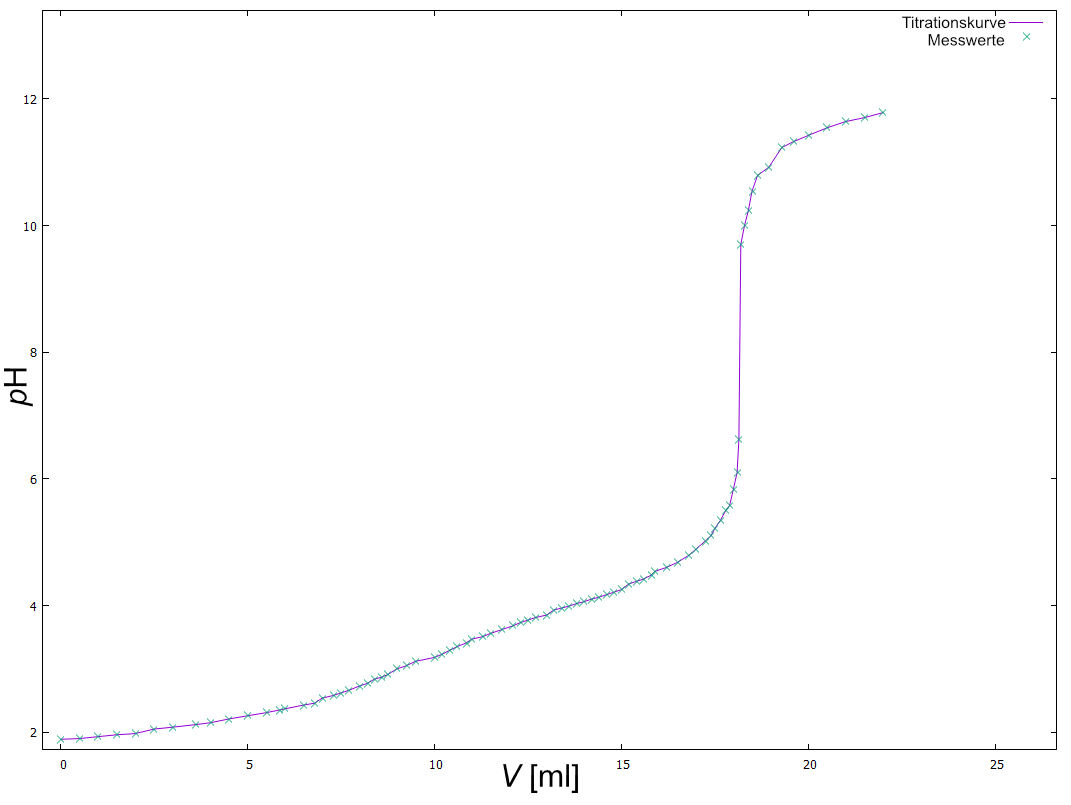
\includegraphics[width=\textwidth]{Abb/oleg.png}\\
    Abb.1: Titrationskurve des ersten Aliquoten.
\end{center}
\begin{center}
    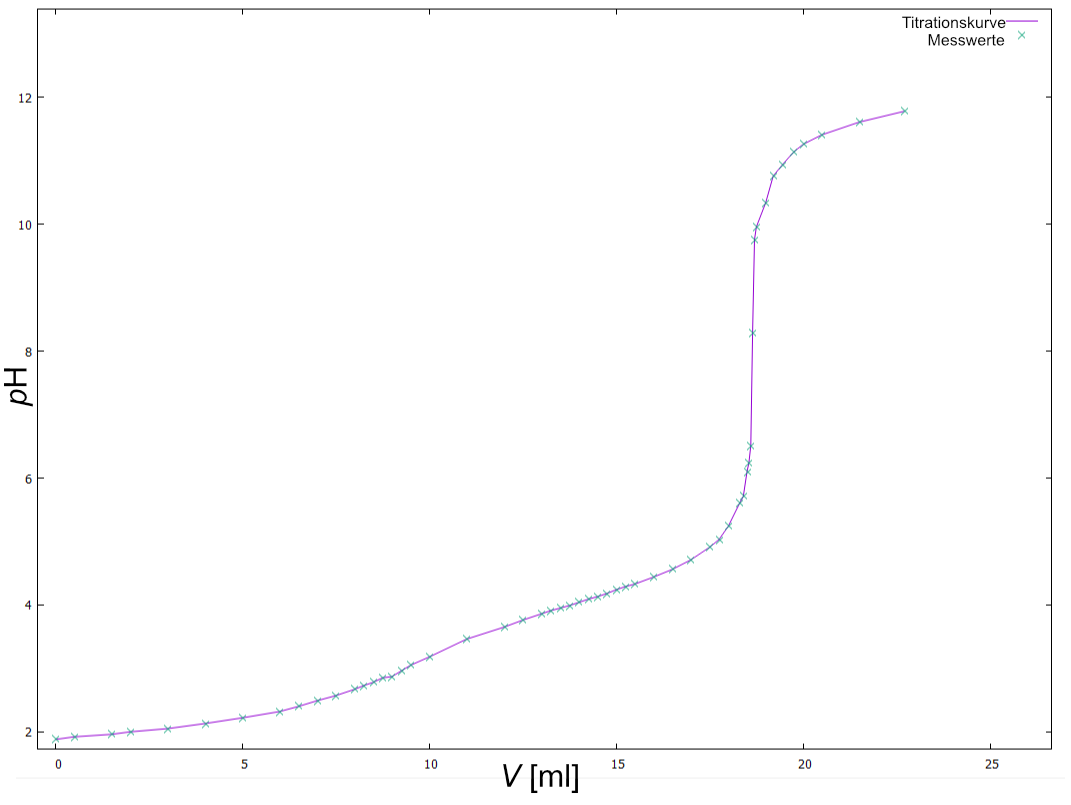
\includegraphics[width=\textwidth]{Abb/oleg2.png}\\
    Abb.2: Titrationskurve des zweiten Aliquoten.
\end{center}
\begin{center}
    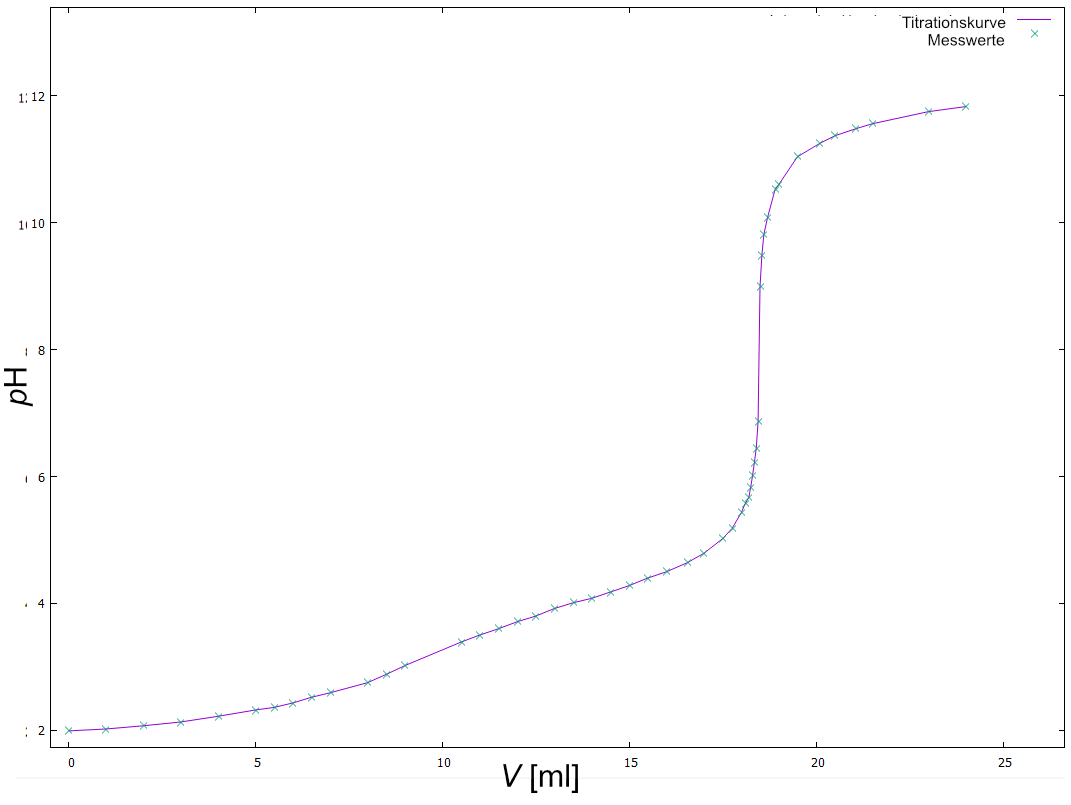
\includegraphics[width=\textwidth]{Abb/oleg3.png}\\
    Abb.3: Titrationskurve des dritten Aliquoten.
\end{center}

Zwar handelt es sich bei der Oxalsäure um eine zweiprotonige Säure, was zwei Umschlagspunkte erwarten lässt, doch der erste konnte nicht auffalend graphisch dargestellt werden.\\
Der zweite und für die Berechnung der Stoffmenge relevante Umschlagspunkt ist hingegen gut zu erkennen und wurde bei den drei Aliquoten auf \\$\Delta V_1 = 18.175\,\mathrm{ml}, \Delta V_2 = 18.65\,\mathrm{ml} \text{ und } \Delta V_3 = 18.5\,\mathrm{ml}$ bestimmt.\\
Mit diesen Werten ist eine Berechnung der Stoffmenge an \ce{NaOH} zu berechnen, die bis zum Umschlagspunkt in die Oxalsäurelösung titriert wurde, wobei $i$ für die Nummer des Aliquoten steht.

\begin{align*}
    n(\ce{NaOH}) &= c(NaOH) \cdot \Delta V_i\\
    &= 0.09321\,\mathrm{\frac{mol}{l}} \cdot 0.018175\,\mathrm{ml}\\
    &= 0.00169409175\,\mathrm{mol}
\end{align*}

Um die Stoffmenge an Oxalsäure zu berechnen wird folgende Formel aufgrund des Zusammenhanges, der aus den Koeffizienten der Reaktanten aus Reaktionsgleichung 1 hervorgeht, verwendet.
\begin{equation}
    \ce{OS_{(aq)} + 2 NaOH_{(aq)} -> OS^{2-}_{(aq)} + 2 Na^{+}_{(aq)} + 2 H2O_{(l)}} 
\end{equation} 
Um den 25 ml Aliquoten auf das Gesamtvolumen von 100 ml zu rechnen, wird mit dem Faktor 4 multipliziert.
\begin{align*}
    n(\mathrm{OS})_1 &= \frac{n(\ce{NaOH})}{2} \cdot 4\\
    &= 2\cdot 1.69409175\,\mathrm{mmol}\\
    &= 3.3882\,\mathrm{mmol}
\end{align*}

Die Berechnung der Sotffmenge der Oxalsäure mit den Werten aus der zweiten und dritten Titration erfolgt analog und liefert die Werte $n_2 = 3.4767\,\mathrm{mmol}$ und $n_3 = 3.3449\,\mathrm{mmol}$\\
Der Mittelwert wird somit wie folgt bestimmt.
\begin{align*}
    n &= \frac{\sum_{i = 1}^{3} n_i}{3}\\
    &= \frac{3.3882\,\mathrm{mmol} + 3.4767\,\mathrm{mmol} + 3.3449\,\mathrm{mmol}}{3}\\
    &= 3.4033\,\mathrm{mmol}
\end{align*}

Somit wurde eine Stoffmenge von $n = 3.4033\,\mathrm{mmol}$ experimentell bestimmt.

\section{Literatur}
[1] Skript zum Praktikum im Modul AC I: 19.07.2023
\end{document}
